\chapter{System Architecture for MT\hyp{}FRHC based G\hyp{}FLCS}

\begin{chapterAbstract}{Preview}
	In this chapter we present a G\hyp{}FLCS architecture and its necessary modules and submodules. The chapter also provides a detailed explanation of a web based user interface for the proposed MT\hyp{}FRHC based G\hyp{}FLCS for reconfigurability. This hardware based fuzzy framework provides online reconfigurability of the system from remote location. However, it is important to note that there are over sixty flexible parameters that needs to be configured and it becomes an arduous task for an user to manage and configure them. Therefore, in this chapter we also introduce a genetic algorithm based parameter extraction technique. This technique helps to develop a course tuning and provide startup parameters which can be later fine tuned by the users remotely through the Web based User Interface. 	
\end{chapterAbstract}
\clearpage

\section{Introduction}
In previous chapter, a MT\hyp{}FRHC based Type\hyp{}I Mamdani G\hyp{}FLCS system is proposed and described.  As discussed briefly in Chapter 2, to counter uncertainty and variations in a nonlinear plant, adaptive control is extremely important. The adaptive control strategy maintains smooth performance of a system in the presence of these uncertainties by updating and tuning FCP at various time intervals. This is implemented in the proposed G-FLCS architecture by introduction of online and offline tuning methods. However, a theoretical analysis of the proposed MT\hyp{}FRHC rule reduction technique is essential before implementation of the tuning methods because the tuning parameters are strictly driven by the active rule reduction mechanism. Subsequently, these modules and submodules gets integrated with G\hyp{}FLCS and analyzed after implementation on a DSP hardware. Earlier in section \ref{sec:obj} it was discussed that \textit{Plug and Play Framework} and \textit{Runtime Tunability} is the essence of G\hyp{}FLCS design. To achieve these key features, it is important to integrate an interactive user interface with the G\hyp{}FLCS design. It is also imperative to formulate the system parameters in accordance to which the G\hyp{}FLCS is to be designed. There are large number of parameters in a Fuzzy Logic Controller. However, a truly generic fuzzy system is impractical because of the fixed resources for implementation. Therefore it is necessary to put an upper bound to each flexible parameter in the Fuzzy Control Parameters (FCP). Nevertheless, unlike most existing G\hyp{}FLCS designs, in this design the number of flexible parameters are not compromised to gain a higher speed. Rather other areas like optimization of code and algorithm is exploited to attain a desired speed and performance. It is also important to note that the FCP driving a G\hyp{}FLCS are generally programmed by users. There are large number of fuzzy parameters for an user to input in the G\hyp{}FLCS. This makes the process quite cumbersome. Hereby, a technique for automatic fuzzy parameter extraction from input\hyp{}output relationship of a process plant will grant the necessary ease of operation for an user. Therefore to start with the design of G\hyp{}FLCS, the system parameters are specified first. 

\section{G\hyp{}FLCS Parameters} \label{sec:des_op}

\begin{table}[b]
	\centering
	\caption{System Parameters}
	\label{tab:sysParam}
	\resizebox{0.65\textwidth}{!}{%
		\begin{tabular}{llc}
			\hline
			\noalign{\vskip 2mm} 
			\multicolumn{2}{c}{\textbf{Parameters}} & \textbf{Values} \\ \hline
			\noalign{\vskip 2mm} 
			\multirow{4}{*}{\textbf{Configurable}} & System Input & 1 to 4 (32 bits) \\
			& number of MFs per I/O & 2 to 7 \\
			& Shape of MFs & \begin{tabular}[c]{@{}c@{}}Triangular, GBell, \\ Trapezoidal, Gaussian\end{tabular} \\
			& Defuzzification Method & Centroid of Area \\ 
			& Rulebase & 2401 ($ 7^4 $)\\ \noalign{\vskip 2mm} \hline
			\noalign{\vskip 2mm} 
			\multirow{3}{*}{\textbf{Fixed}} & System Output & 1 \\
			& Method & MIN-MAX \\
			& I/O Signal Range & -5 to +5 V \\ \noalign{\vskip 2mm}  \hline
			
		\end{tabular}
	}
\end{table}
To start with the design of G\hyp{}FLCS, the system parameters are specified first. The FCP of proposed G\hyp{}FLCS is segregated into two segments namely configurable parameters and fixed parameters. Table \ref{tab:sysParam} presents the features of the proposed G\hyp{}FLCS. This table presents configurable and non\hyp{}configurable (fixed) parameters along with  order and variable values for a four\hyp{}input and one\hyp{}output system. Characteristics features of this architecture is as follows: 
\begin{itemize}
	\item A 32 bit precision Input and Output is considered.
	\item A web based user interface (WebUI) to remotely acquire fuzzy parameters. 
	\item Wide range of output MFs tuning consisting of singleton, triangular, trapezoidal, Gaussian and GBell type membership functions.
	\item MIN\hyp{}MAX Inference with full set rules.
\end{itemize}
This controller was implemented on a TI C6748 DSP processor. The major reasons for using DSP are:
\begin{itemize}
	\item DSP provides an effective implementation of multiplication and accumulation (MAC) and this helps in efficient COA implementation.
	\item File handling and socket programming is an integral part of this design. These were achieved easily since the development is in C language.
	\item This design supports high level of branching and decision making.
\end{itemize}	 

\section{System Architecture of Proposed G\hyp{}FLCS}
The proposed system architecture involves hardware\hyp{}software co\hyp{}design to present a complete reconfigurable G\hyp{}FLCS as shown in Figure \ref{fig:ProposedFLCArchitecturalDesign} and Figure \ref{fig:ProposedGenericFuzzyLogicSystemArchitecture}. In Figure \ref{fig:ProposedFLCArchitecturalDesign}, a graphical abstract of the overall system is represented. It can be observed that the controller is interfaced on one side in a feedback loop with the plant and on other side with the users through a client\hyp{}server based interface. The client\hyp{}server model allows reconfigurability of the system from remote locations. Figure \ref{fig:ProposedGenericFuzzyLogicSystemArchitecture} presents the internal architecture of the G\hyp{}FLCS design.  

The WebUI in client server model represents the software and the driver layer to interface the hardware G-FLCS through serial port to the server. The DSP hardware receives FCP data serially and stores them in predefined memory locations. These parameters are segregated in two categories namely \textit{Setup}  parameters and \textit{Rulebase} data. The driver layer in the hardware G\hyp{}FLCS receives and acknowledges the data transmission. 
A WebUI drives the proposed hardware G\hyp{}FLCS storing FCP data in a file in specific format. The file is shown in Appendix-A. It may be noted that the FCP file is generated deliberately in accordance with Matlab Fuzzy Inference System (FIS) file format to provide liberty to integrate a parameter data file generated using Matlab Fuzzy Logic Toolbox as well. Submitting the parameters triggers a desktop application that is native to the server. Objective of this program is to transmit the FCP from database to the hardware G\hyp{}FLCS through serial communication. The FCP data is stored in the DSP board based according to a predefined memory map. G\hyp{}FLCS designed with MT\hyp{}FRHC rule reduction scheme, operates on the inputs with these FCP data to provide desired control action. Fuzzifier, inference engine and defuzzifier is programmed with information about the data and its corresponding memory location. With these information, fuzzifier transforms crisp inputs in fuzzy domain and a Mamdani inference engine, coupled with the Rulebase in the system memory produces fuzzy output. Defuzzifier transforms the fuzzy output compiled by the inference engine to provide crisp output. There are various types of defuzzifier but in this work centroid of area (COA) is used considering its popularity and effectiveness. 

%Offset address \textbf{0000}H to \textbf{00D6}H in Table \ref{tab:memorymap} shows the details of Setup parameters. \textit{Rulebase} parameters appear in memory location \textbf{00D7}H to \textbf{1D0C}H which is reserved to store \textbf{{2401}\footnotemark} ~rules.
%\footnotetext{Maximum number of rules that this design can support is ($ = 7^4 $) since there can be maximum of 7 MFs for maximum of 4 Inputs.} 
\begin{figure}[h!]
	\centering	
	\subfloat[System Architecture]{\label{fig:ProposedFLCArchitecturalDesign}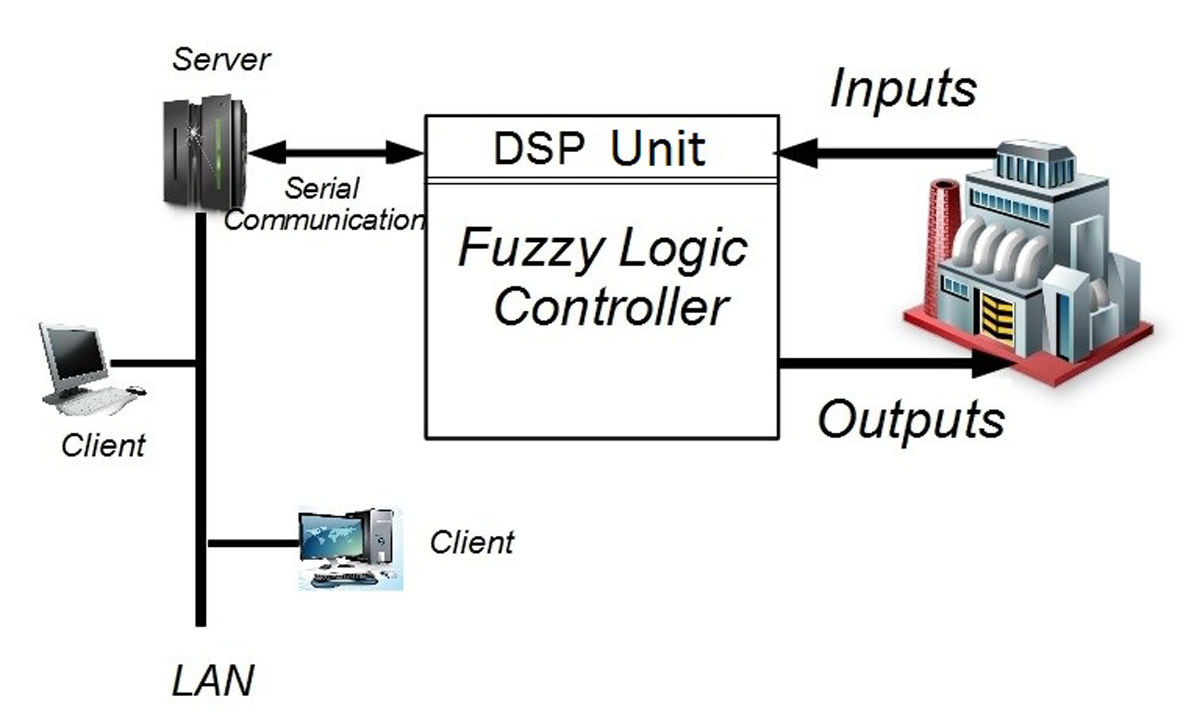
\includegraphics[width=0.9\linewidth]{Chapter3/chapter3/Fig1.eps}} \\
	\subfloat[Hardware Design]{\label{fig:ProposedGenericFuzzyLogicSystemArchitecture}\includegraphics[width=0.9\linewidth]{Chapter3/chapter3/Fig2.eps}} 
	\caption{Proposed G-FLCS Design Architecture}
	\label{fig:sysArch}
\end{figure}
\section{Development of a Client\hyp{}Server Model User Interface} \label{sec:WebUI}
A client\hyp{}server model is widely used for data transfer over large distance. Computer applications like are Email, network printing, and the World Wide Web use client–server model for data exchange. It is reliable, fast and secured distributed application structure. In the proposed design, it is cardinal to have a distribution structure over which users from large distance can operate the controller. 
\subsection{client\hyp{}server Model}
The client\hyp{}server model, also known as server\hyp{}client model, is a computing model developed on distributed computing structure. This structure segregates workload between a centrally connected service provider (\textit{Server}) and the various service users (\textit{Clients}) \cite{Simon2006}. Its is a standard model for developing network applications. The \textit{Server} process starts the computing module by initializing itself. Once the initialization protocol successfully completes, it goes to sleep and waits for incoming client requests. \textit{Client} processes can initiate from any system in the network including the host system running the \textit{Server} process. Once a service request is attended, this \textit{Server} application goes back to sleep and awaits incoming requests. 
Server applications or processes are of two types.
\begin{itemize}
	\item \textbf{Iterative:} In these type of applications, a single copy of the server application executes to service only a single user at any time. While a user request is attended, other users have to wait. These applications are developed when prior knowledge about the time to service individual request is present. 
	\item \textbf{Concurrent:} These \textit{Server} applications provides service to multiple users at any time. When a user requests for a service, the \textit{Server} application replicates a copy of itself which dedicatedly serves that user. This process repeats for every incoming service requests from the \textit{Clients}. These applications are developed when prior knowledge about the time to service individual request is absent.	
\end{itemize}
The client\hyp{}server model of communication developed for hardware G-FLCS uses TCP. TCP is an important protocol of TCP/IP networks where it helps to establish connection and exchange data. Establishment of a connection between two hosts depends upon five components
\begin{itemize}
	\item Protocol used
	\item Source IP address
	\item Source port number
	\item Destination IP address
	\item Destination port number 
\end{itemize}
With proper set of information, a connection between two hosts is established.

\subsection{ASP.NET and development of WebUI}
In this work, ASP.NET has been extensively used to develop the WebUI for hardware G-FLCS. This web application is designed with an intention to develop an user interface which, once installed on a central server, can be accessed over Internet to provide remote reconfigurability to the proposed hardware G-FLCS. The framework behind this application is demonstrated pictorially in Figure \ref{fig:fig3_9}. The figure shows that Microsoft IIS7 hosts and web application and interfaces it to the internet. Users from different location can access this application. Standard IP protocols are used for the WebUI for hardware G-FLCS as stated in Table \ref{tab:protocols}
\begin{table}[t]
	\centering
	\caption{TCP/IP Communication Layers and their Protocols}
	\label{tab:protocols}
	\begin{tabular}{ccc}
		\hline SL. No. & Layer & Protocol \\ 
		\hline 1. & Data Link Layer & Ethernet \\ 
		2. & Network Layer & IP \\ 
		3. & Transport Layer & TCP \\ 
		4. & Application Layer & HTTP \\ 
		\hline 
	\end{tabular} 
\end{table}
Here the WEBUI is hosted on a PC with IP address 192.168.50.102. Using HTTP, users can access the WebUI over Internet upon request and authentication. Since this application is time critical and sensitive to FCP data, it is important to develop it as an iterative server application which automatically limits user to one. Microsoft IIS7 has been used for web-server and it can host web applications developed on ASP.NET framework. This was a major motivation of using ASP.NET for developing this application. A user request is processed by IIS and it passes the request to the web application WebUI, which generates response in HTML and returns it to IIS. Thereafter, IIS returns this HTML response to the user initialing the request.
\begin{figure}[h!]
\centering

\includegraphics[width=1\linewidth]{Chapter3/chapter3/Fig9}
\caption[Framework behind WebUI for hardware G-FLCS]{Framework behind WebUI for hardware G-FLCS}
\label{fig:fig3_9}
\end{figure}
 
\subsection{WebUI for Hardware G-FLCS}
\begin{figure}
	\centering
	\subfloat[Basic Parameters]{\label{fig:BasicParameters}\includegraphics[scale=0.38]{Chapter3/chapter3/Fig3.eps}} \\
	\subfloat[Input Membership]{\label{fig:InputMembership}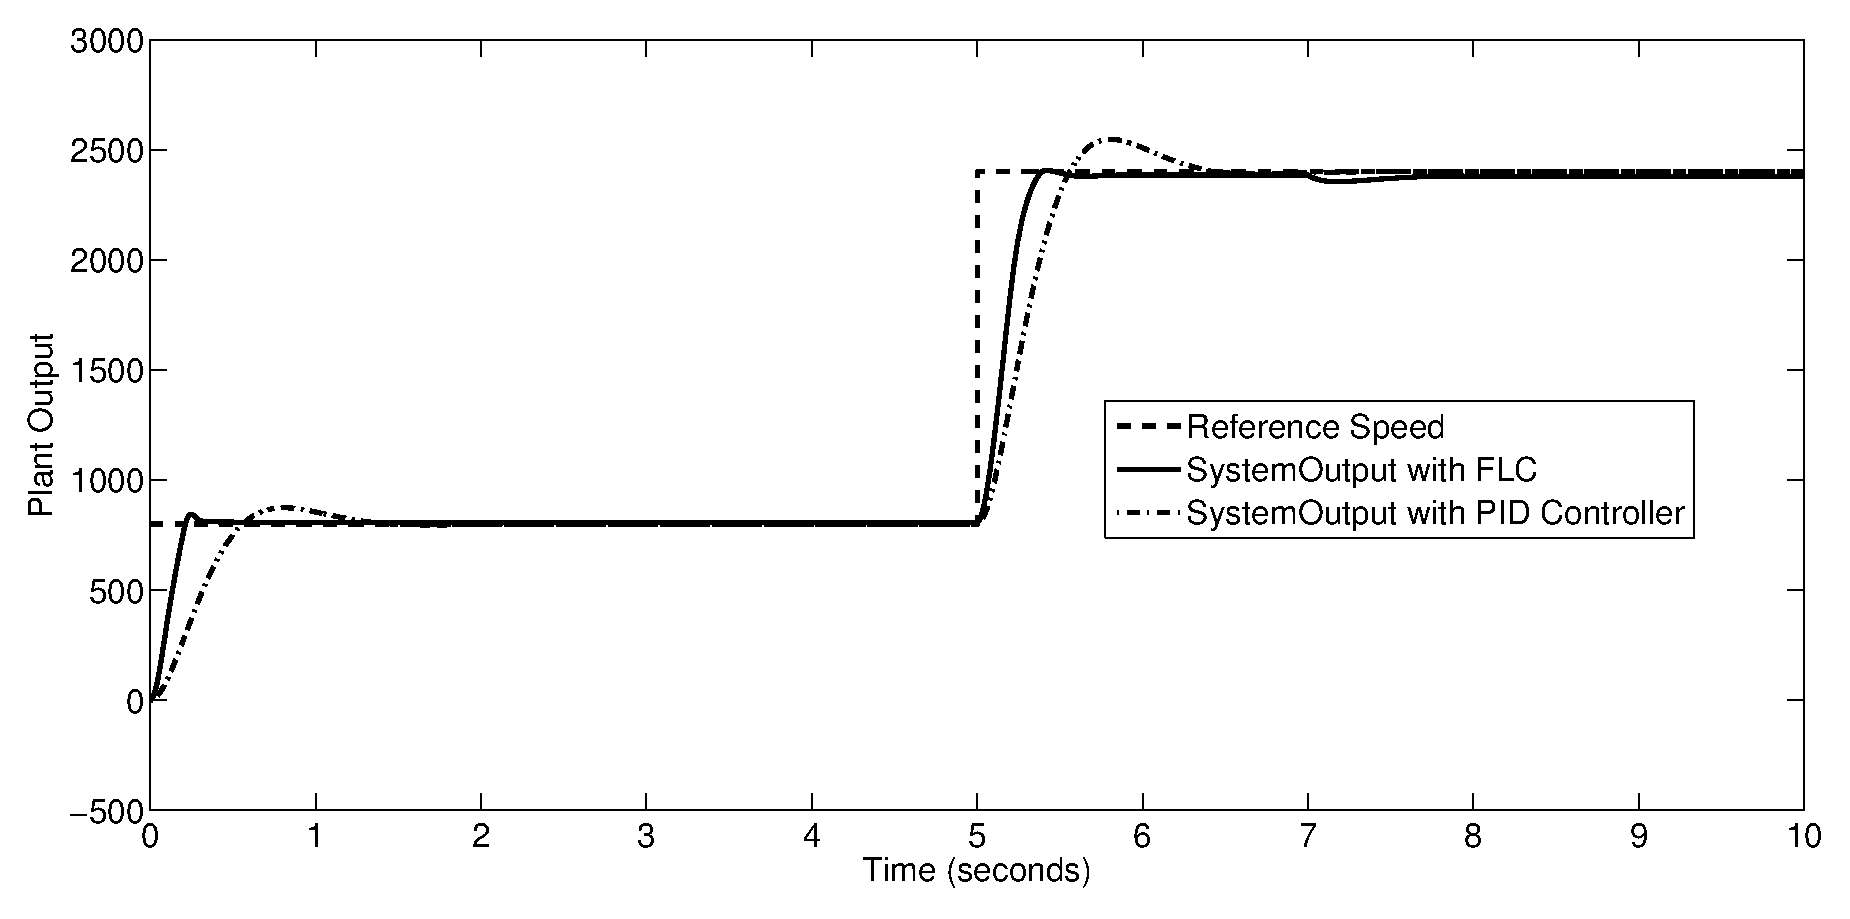
\includegraphics[scale=0.38]{Chapter3/chapter3/Fig4.eps}} 
	\caption{WebUI for Hardware G-FLCS developed using ASP.NET with C\# and hosted using Microsoft IIS7}
	\label{fig:WebUI}
\end{figure}
\begin{figure}
	\centering
%	\ContinuedFloat 
	\subfloat[Output Membership]{\label{fig:OutputMembership}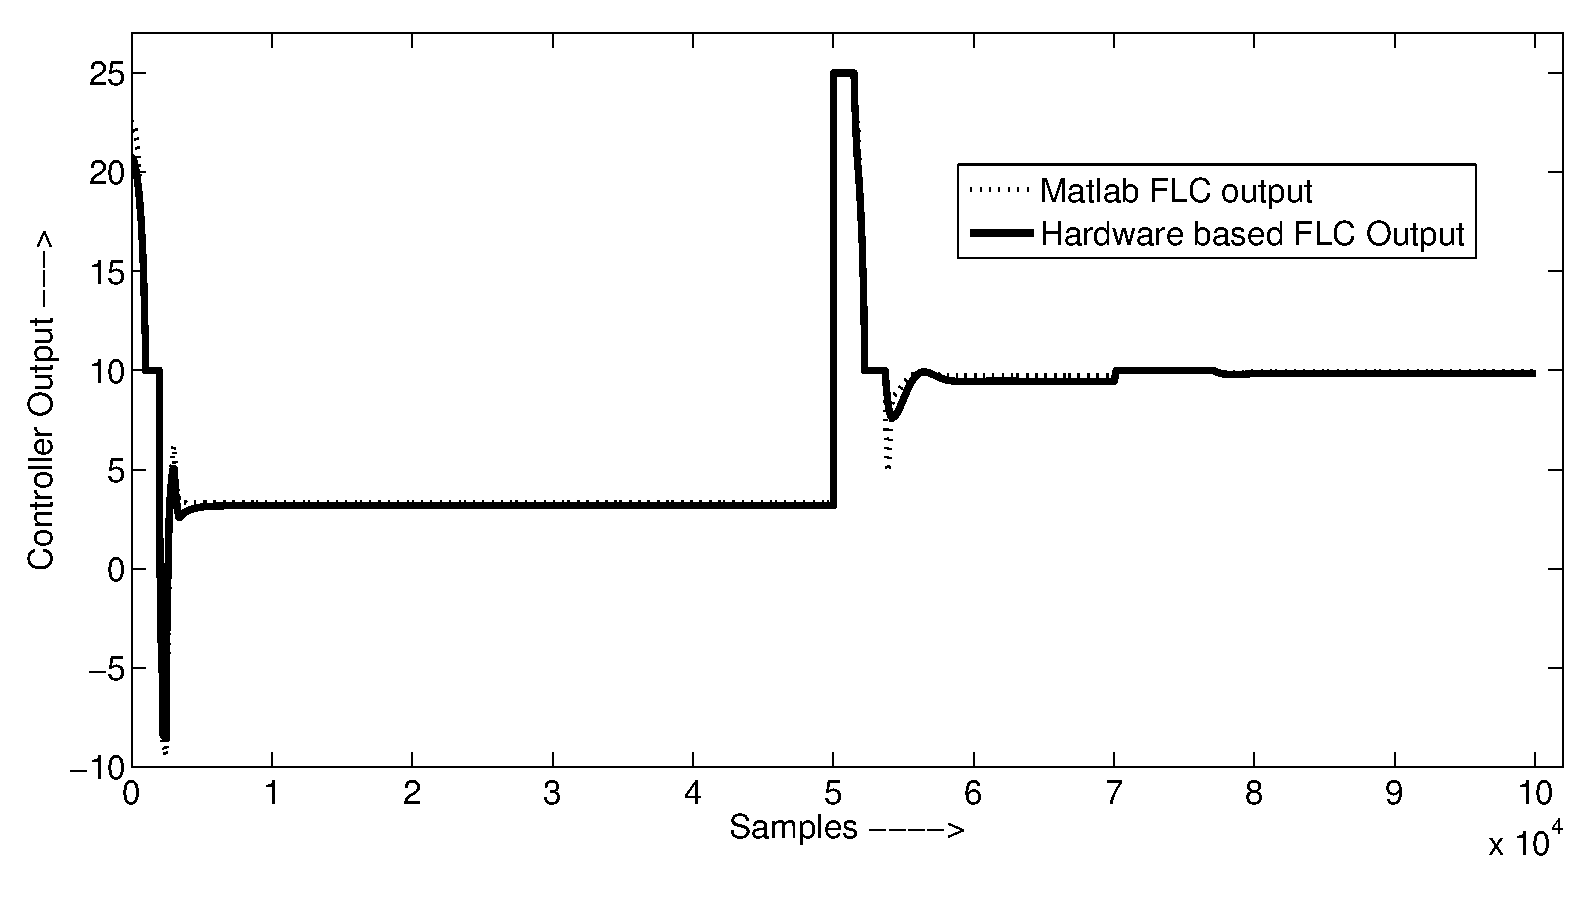
\includegraphics[scale=0.38]{Chapter3/chapter3/Fig5.eps}} \\
	\subfloat[Rulebase]{\label{fig:RuleBase}\includegraphics[scale=0.38]{Chapter3/chapter3/Fig6.eps}} 
	\caption{WebUI for Hardware G-FLCS developed using ASP.NET with C\# and hosted using Microsoft IIS7}
	\label{fig:WebUI2}
\end{figure}
\par
WebUI is developed in ASP.NET with C\# and deployed using Microsoft IIS-7. The Web Pages that serves to collect various information pertaining to parameters related to FLC from users are shown in Figure \ref{fig:WebUI} and Figure \ref{fig:WebUI2}. Web page in Figure \ref{fig:BasicParameters} presents the WebUI where, parameters like \textit{name}, \textit{type}, \textit{implication}, \textit{aggregation}, \textit{and} method,\textit{ or} method and \textit{defuzzification} type are defined. Web page in Figure \ref{fig:InputMembership} accepts details of inputs and their MFs whereas Web page in Figure \ref{fig:OutputMembership} accepts details about outputs and their corresponding MFs. Web page in Figure \ref{fig:RuleBase} accepts the Rulebase and stores all data in FCP file as mentioned in Appendix. On submission, these information data are validated and a server application for communication with the board is invoked. This WebUI can be accessed over Ethernet from a client system situated far away from the controller and plant (simulated model).

\section{Genetic Algorithm based Fuzzy Parameter Extraction} \label{sec:FCP}
A genetic algorithm (GA) is a search heuristic that mimics the process of natural selection and has been widely used evolutionary method for optimization of FLCs, both type I and II\cite{Ishibuchi1995a,Shopova2006,Bandyopadhyay2001a,Maldonado2014,Alcala2006a,Sanz2011}. This technique has been widely used in the literature for fuzzy optimization. Other popular methods for fuzzy optimization are Univariate Marginal Distribution Algorithm (UMDA)\cite{bookBehera2009}, stochastic Hill Climbing(SHC) \cite{Michta2011,Chen2003a}, Baysian Optimization Algorithm (BOA) \cite{Jiang2000}. 
\begin{table}
	\centering
	\caption{Genetic Algorithm Parameters}
	\label{tab:GS_Param}
	\begin{tabular}{cc}
		\hline Parameters & Value/Function \\ 
		\hline Population & 120 \\ 
		Generation & 200 \\ 
		Fitness Scaling & Rank \\ 
		Selection & Stochastic \\ 
		Crossover Probability & 0.8 \\ 
		Elite Count & 6 \\ 
		Mutation Function & Adaptive feasible  \\ 
		Crossover Function & Adaptive feasible  \\ 
		Stopping Criteria & Fitness Limit \\ 
		\hline 
	\end{tabular} 
\end{table}

\begin{figure}[h!]
	\centering
	
\includegraphics[width=0.85\linewidth]{Chapter3/chapter3/Fig7_offline.eps}
	\caption{Fuzzy Control Parameter (FCP) extraction using Genetic Algorithm}
	\label{fig:fig3_7}
\end{figure}
Response from a system with maximum of four inputs and one output is recorded. Once the dataset is derived, it is passed on to the system for FCP extraction. The proposed method for FCP extraction is based on Genetic Algorithm. Details of the parameters used in Genetic Algorithm is displayed in Table \ref{tab:GS_Param}. There are 60 system parameters that are optimized using genetic algorithm to achieve two objectives, namely
\begin{itemize}
	\item Quick settling, and
	\item Tracking reference.
\end{itemize}
Figure \ref{fig:fig3_7} portrays basic blocks of a Genetic Algorithm based FCP extraction technique. An initial set of random parameters are input to the Genetic Algorithm system. Every optimization technique operates on a cost function. The cost function can be represented by the process plant simulation model or its I/O dataset. The FCP parameters are manipulated such that a set of optimized FCP is obtained which provide quick settling and fast reference tracking.  
The Simulink model with initial FCP is used as an objective function which returns the transient and settling time. The co-ordinates of the membership functions are treated as the nonlinear inequality constraints. Thus varying these FCP will provide with an absolute tracking of reference\footnote{The codes can be downloaded from \url{https://goo.gl/Zb17fZ}}.

\section{Data flow of the proposed system}
\begin{figure}[h!]
	\centering
	\includegraphics[width=1\linewidth]{Chapter3/chapter3/Fig8.eps}
	\caption{Dataflow of the proposed G-FLCS system}
	\label{fig:fig3_8}
\end{figure}
In this implementation process, data synchronization and communication between user and the hardware G-FLCS is critical. The process is presented in Figure \ref{fig:fig3_8}. This figure depicts how data communication is achieved with the help of various control signals between, client-server and server-GFLCS. The web application provides a systematic user interface which collects data from authenticated users. The application waits for a new connection request on startup. On successful login, the user is presented with a web page containing four different tab-windows, each for basic parameters, information about inputs, outputs and Rulebase. These windows are preloaded with extracted parameters as presented in Figure \ref{fig:fig3_7} and provide a way for fine tuning the control parameters by an operator. In Figure \ref{fig:fig3_8}, operations like connections, login, parameter collection and communication with hardware G-FLCS through a server program are performed by the web application and are shaded in \textit{Light Grey}. 
When a user provides the fuzzy control parameters (FCP) data, the web application validates the entered data based on following protocols.
\begin{itemize}
	\item All MFs have properly defined co-ordinates within specified range of operation.
	\item Number of Input(s) and Outputs are correctly defined. 
	\item Rules are validated according to Mamdani model.
\end{itemize}
After validation of new parameters, the server application connects serially to the hardware G-FLCS. Serial communication protocol has been used here for the ease of implementation. This data communication can be easily extended to industry standard controller area network (CAN) protocol. G-FLCS completes current execution and generates control signal to the system. Thereafter, it acknowledges any incoming serial communication request and starts receiving and storing fuzzy parameters in the data memory. Sys/BIOS is widely used real time operating system for TI DSPs and has been used in this work to take care of the multitasking of fuzzy processes.


\section{System Integrity Test}
To provide proof of concept for this proposed design, an experiment was carried out with an Intel Corei5-2400 3.1 GHz PC with 4GB memory operating as a server with the WebUI. It is available to all the clients in the local network over same gateway. Authenticated user loads FCP data in a text file located in the server. 

\begin{figure}[h!]
	\centering
	\subfloat[Plant Output: Two Tank Water Level System]{\label{fig:TT_Out}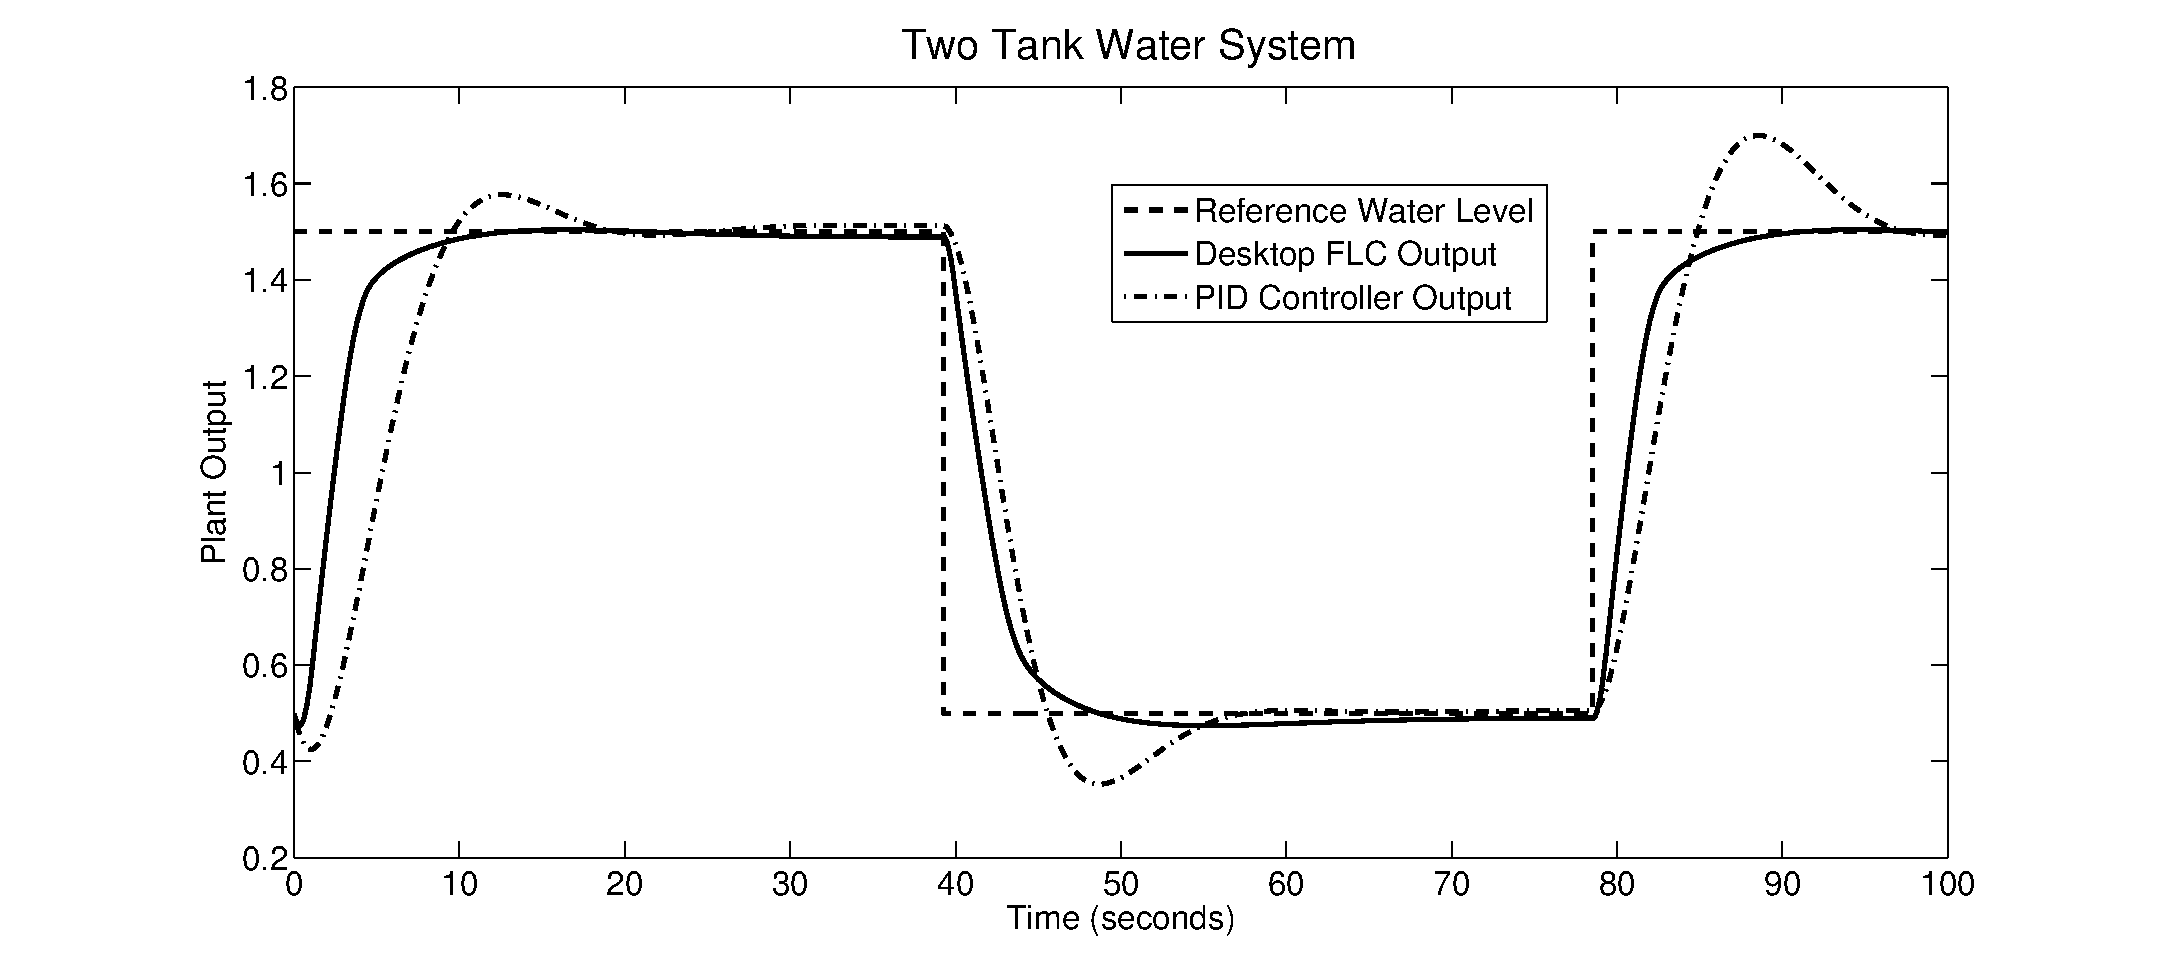
\includegraphics[width=0.9\linewidth]{Chapter3/chapter3/TankPO.eps}} \qquad
	\subfloat[Controller Output: Two Tank Water Level System]{\label{fig:TT_Con}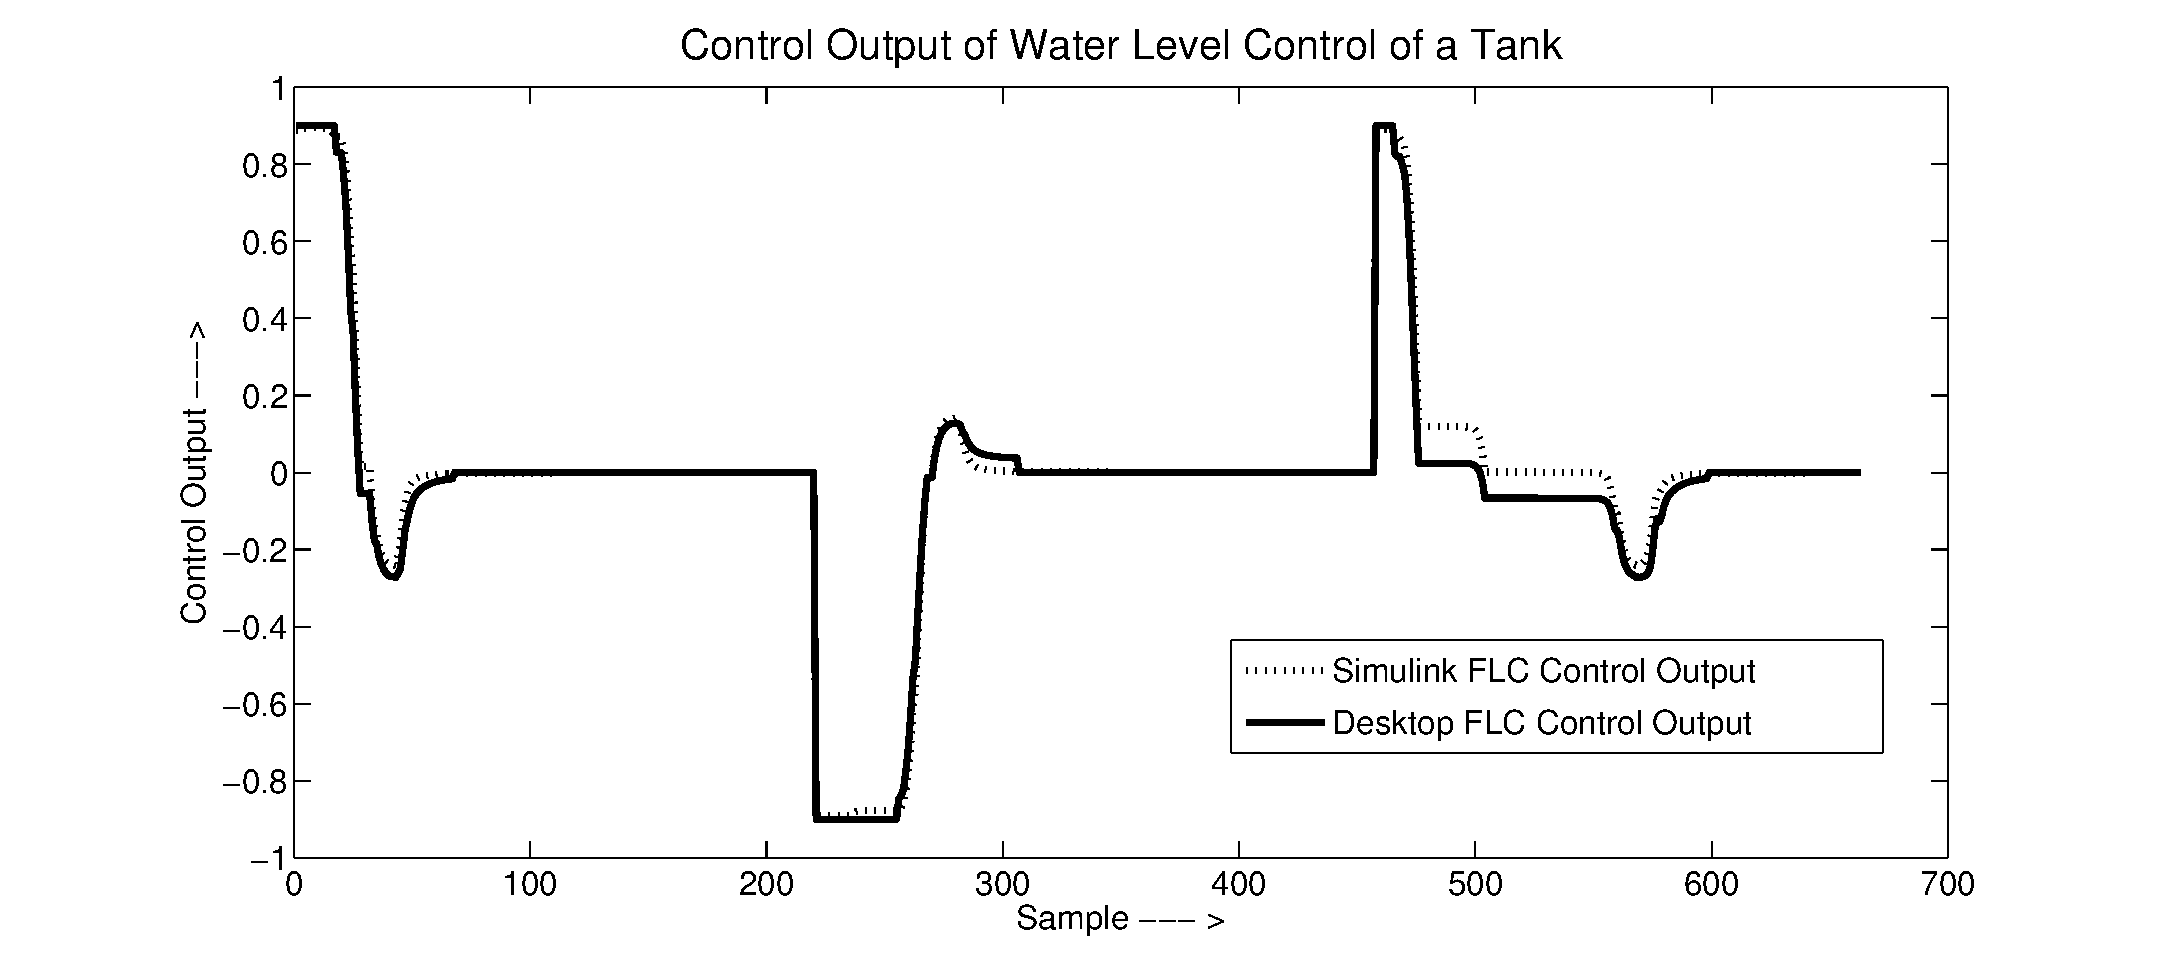
\includegraphics[width=0.9\linewidth]{Chapter3/chapter3/TankCO.eps}}
	\caption{Plant output and Controller output of various test models. The controller output is a comparison between output from Matlab Fuzzy Logic Toolbox and proposed hardware G-FLCS. Plant output shows performance of the proposed FLC structure with PID controllers conducted using through HIL testing environment} 
	\label{fig:CompOut_tank}
\end{figure}

\begin{figure}[h!]
	\centering
	\subfloat[Plant Output: Intelligent Cruise Control System]{\label{fig:ICC_Out}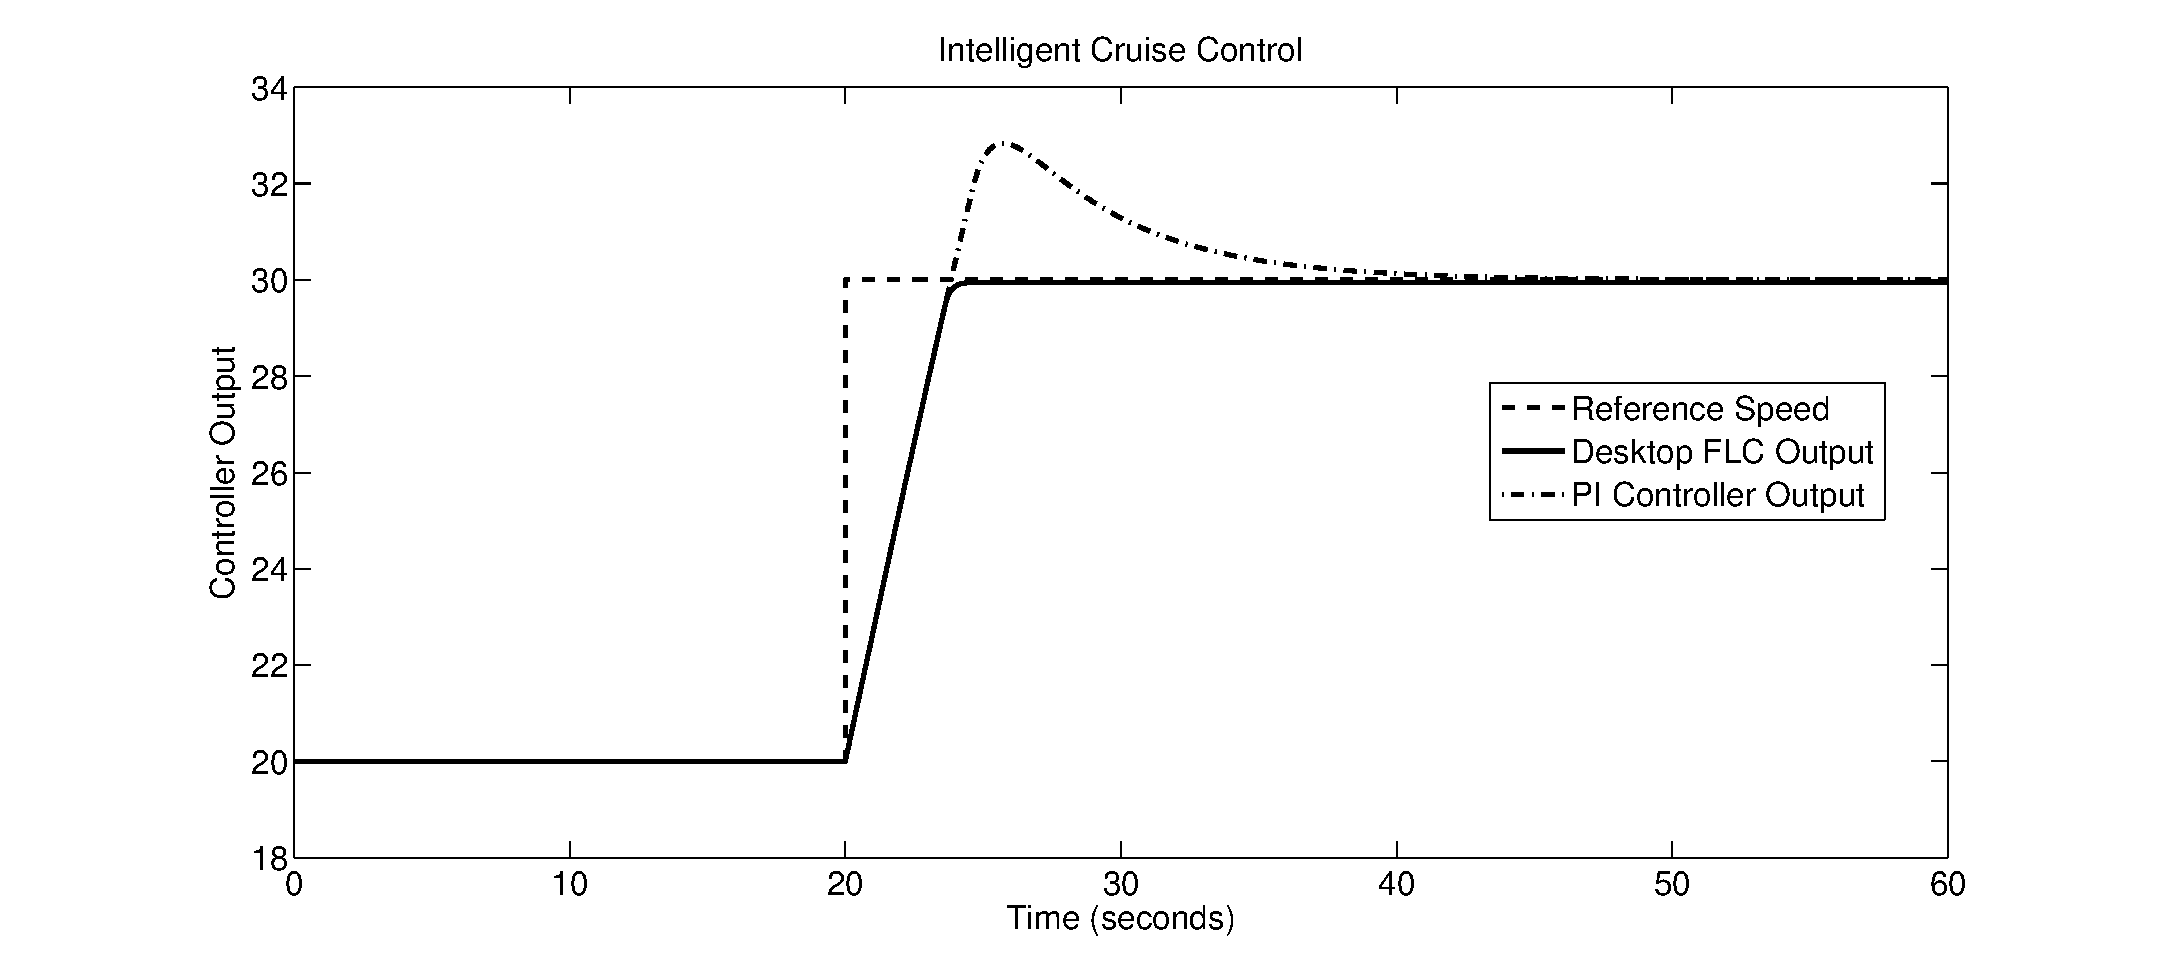
\includegraphics[width=0.9\linewidth]{Chapter3/chapter3/IccPO.eps}}\\
	\subfloat[Controller Output: Intelligent Cruise Control System]{\label{fig:ICC_Con}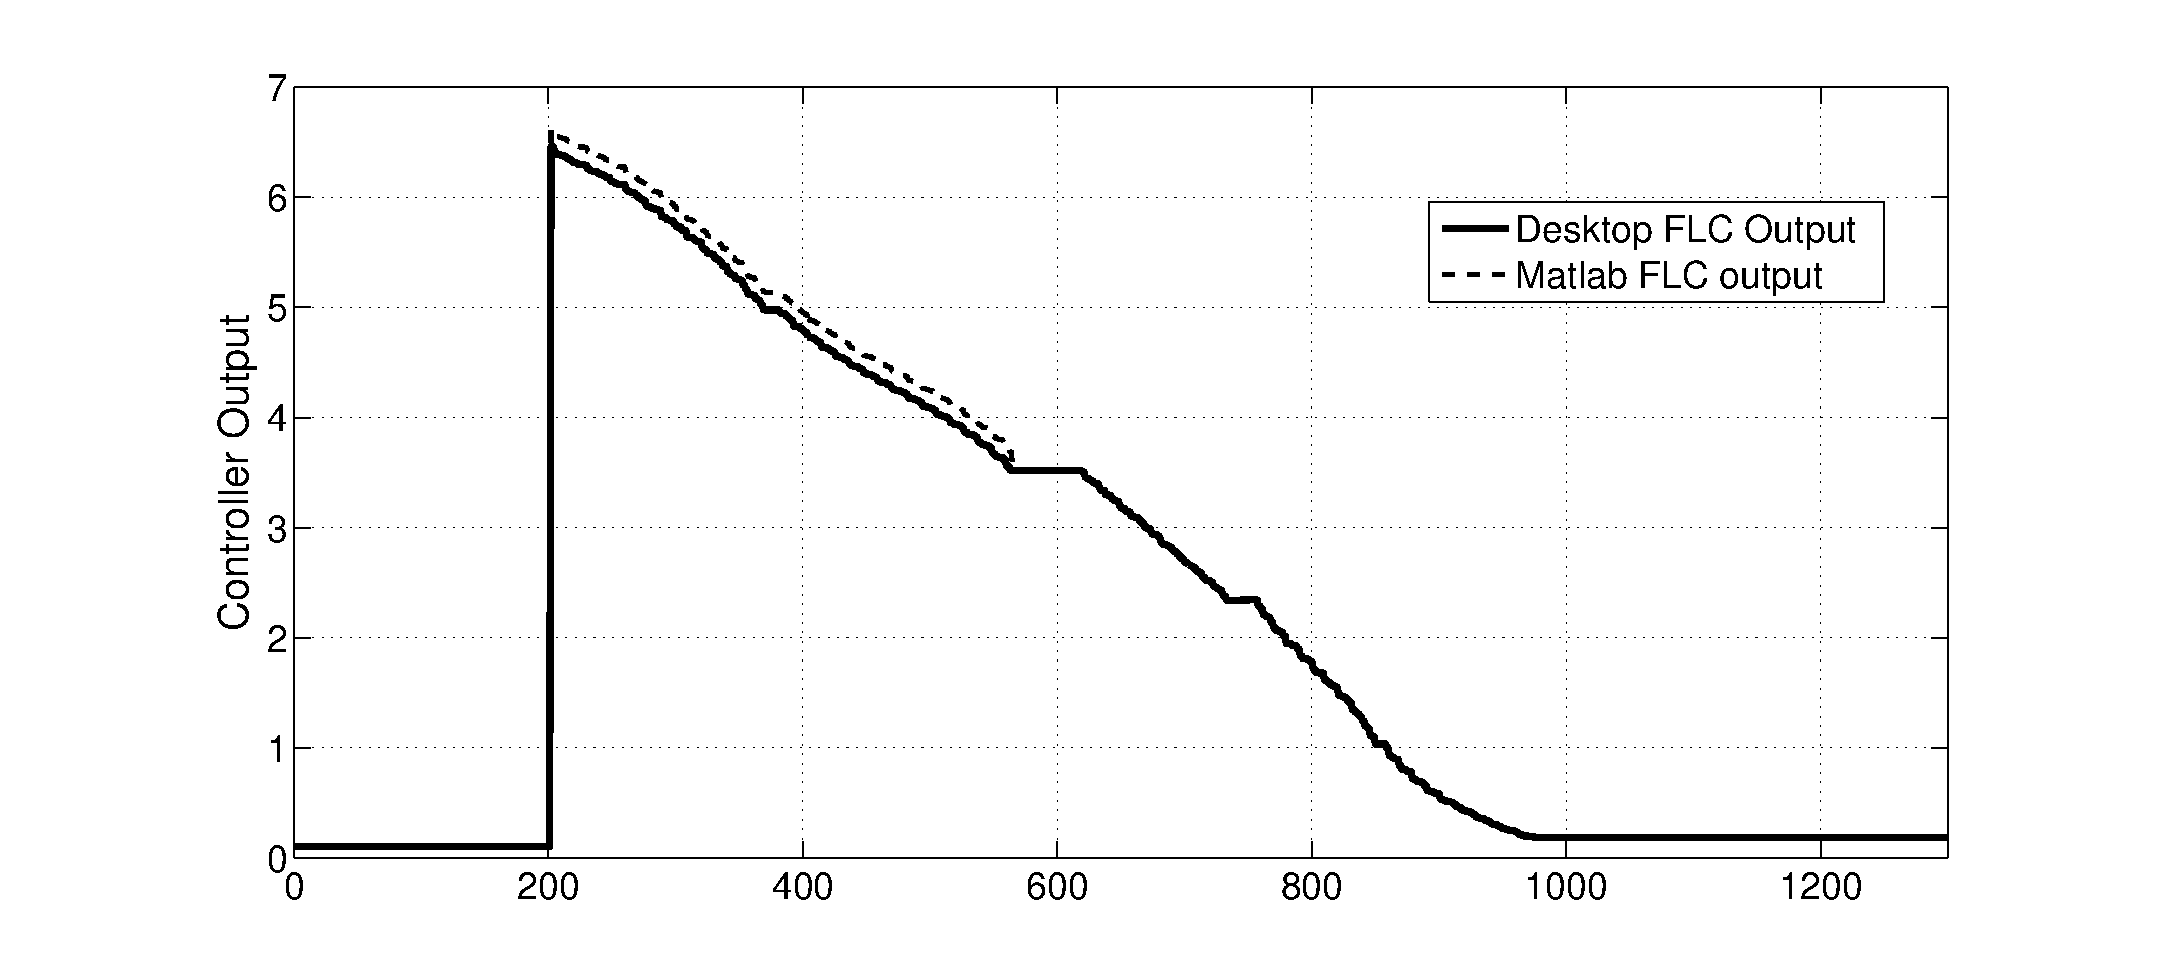
\includegraphics[width=0.9\linewidth]{Chapter3/chapter3/IccCO.eps}}
	\caption{Plant output and Controller output of various test models. The controller output is a comparison between output from Matlab Fuzzy Logic Toolbox and proposed hardware G-FLCS. Plant output shows performance of the proposed FLC structure with PID controllers conducted using through HIL testing environment} 
	\label{fig:CompOut_icc}
\end{figure}


\begin{figure}[h!]
	\centering
	\subfloat[Plant Output: First-order system with dead time for anti-windup scheme]{\label{fig:AWU_Out}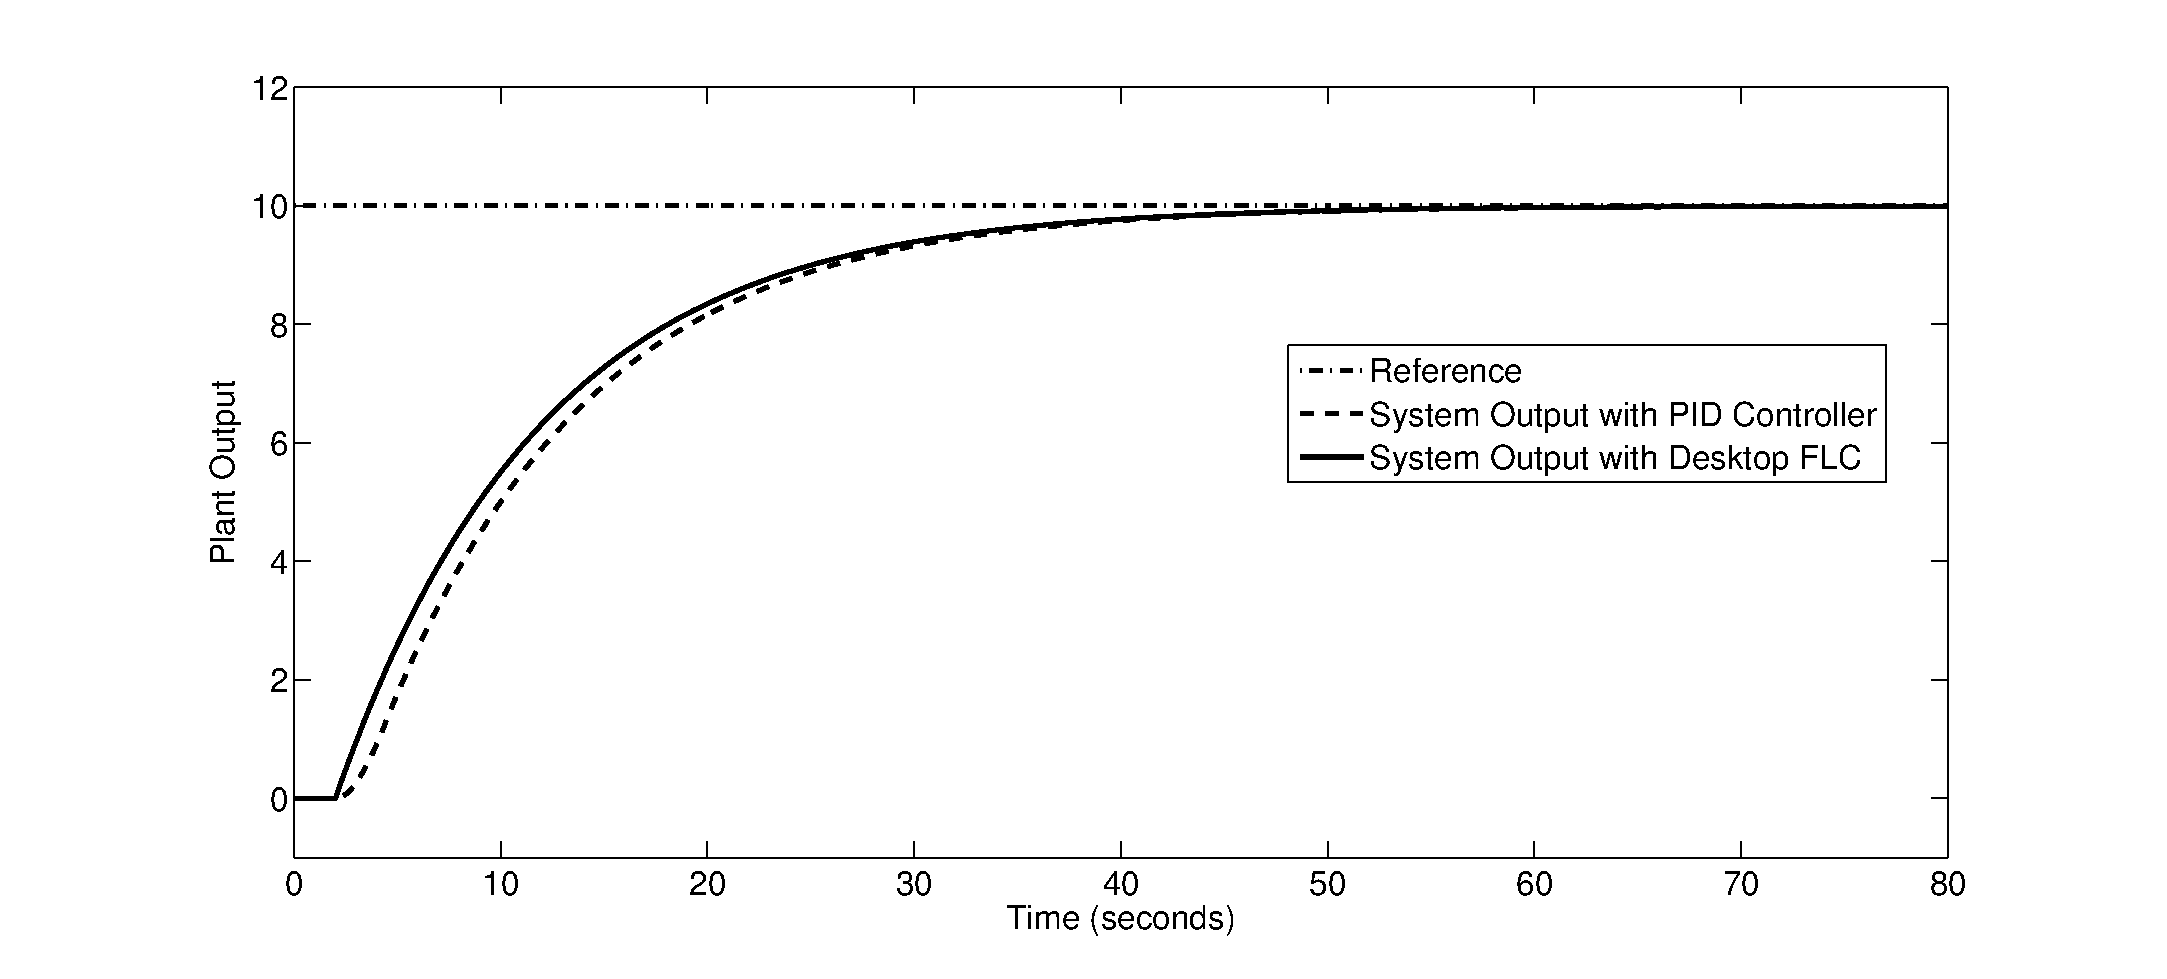
\includegraphics[width=0.9\linewidth]{Chapter3/chapter3/AwbPO.eps}} \qquad 
	\subfloat[Controller Output: First-order system with dead time for anti-windup scheme]{\label{fig:AWU_Con}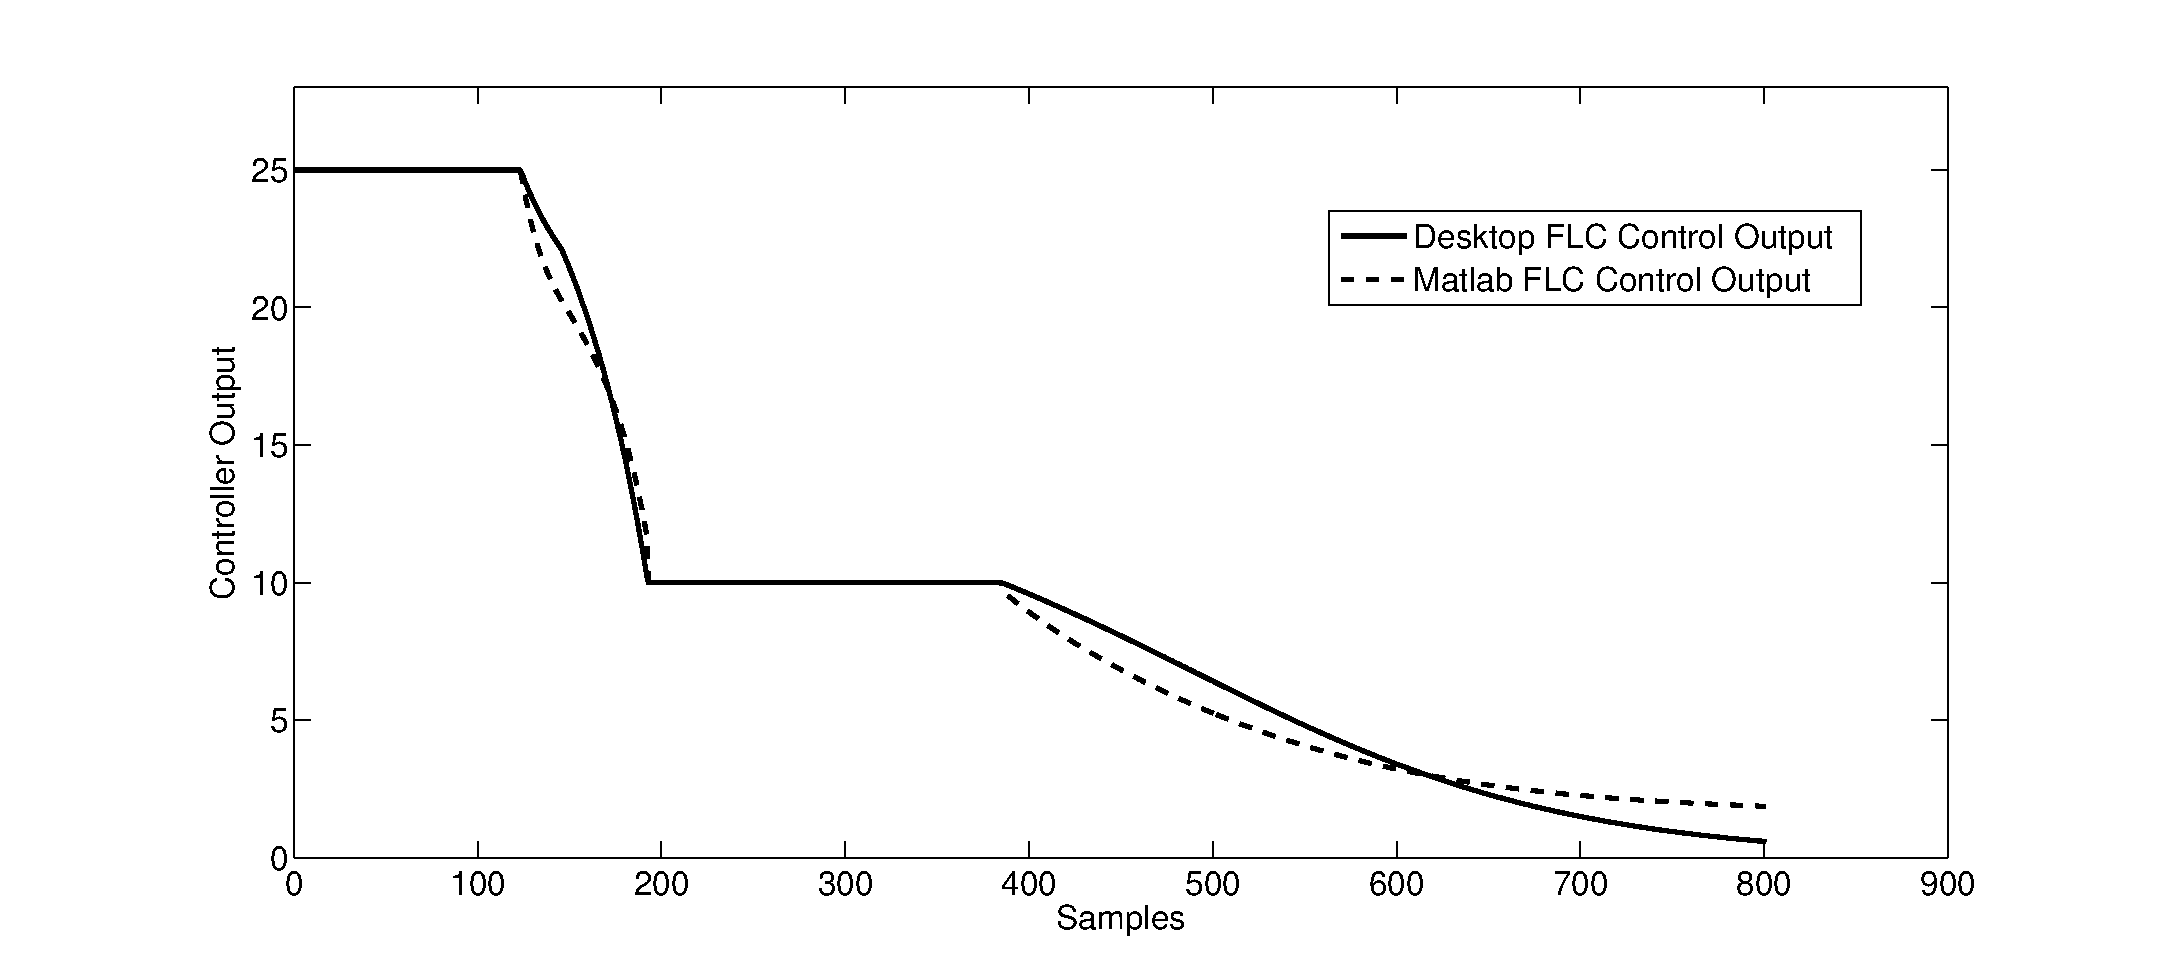
\includegraphics[width=0.9\linewidth]{Chapter3/chapter3/AwbCO.eps}}
	\caption{Plant output and Controller output of various test models. The controller output is a comparison between output from Matlab Fuzzy Logic Toolbox and proposed hardware G-FLCS. Plant output shows performance of the proposed G-FLCS structure with PID controllers conducted through HIL test environment} 
	\label{fig:CompOut_wind}
\end{figure}

The code developed for hardware G-FLCS is compiled using MS Visual Studio to generate a desktop application which runs on the server and mimics the hardware G-FLCS. This FCP data is used by desktop FLC to generate control signal. Plant models are developed in Matlab and communicates with the desktop FLC using $ system $ command. The functionality is executed in following steps:
\begin{description}\label{algo:StepsSim}
	\item[Step 1] Generation of I/O dataset from Simulink model using PID controller.
	\item[Step 2] Apply GA based FCP extraction algorithm described in section \ref{sec:FCP}, to extracted FCP from the I/O dataset generated in Step 1. 
	\item[Step 3] Appropriate FCP data is programmed through WebUI and submitted to the server.
	\item[Step 4] The plant model is executed with the stored FCP. For controlling the plant, Matlab uses $ system $ command to invoke the desktop FLC program and passes the FCP and input data \_IN as arguments. Desktop FLC computes and returns the output to Matlab. This forms the controller output.
	\item[Step 5] The Simulink plant output is computed with controller output. It is stored and plotted with respect to plant output using PID controllers for comparative analysis.
	\item[Step 6] The dataset is used to compare the control signal from desktop FLC to control signal from Matlab Fuzzy Inference System for performance analysis.
\end{description}
 
Some benchmark control problems were used to test the applicability and generality of the proposed architecture, namely Two Tank Water Level Controller \cite{twotank2012,Laubwald2006}, Intelligent Cruise Control \cite{Naranjo2003}, first order system with dead time for anti-windup scheme \cite{antiwindup2014}. All these system models were implemented on Simulink and they are available in Mathworks File Exchange repository. The integrity of the proposed architecture is tested with these models according to the algorithm described above. In Figure \ref{fig:CompOut_tank}, Figure \ref{fig:CompOut_icc} and Figure \ref{fig:CompOut_wind} the observed results from these simulated tests are displayed. The proposed MT-FRHC based Web Configurable G-FLCS is implemented on the desktop server using C code interface by an application program to the WebUI. This provides a platform for evaluation of the proposed technique before it is realized on actual hardware platform. In Figure \ref{fig:TT_Out}, the plant output of this proposed desktop G-FLCS is compared to a tuned PID controller when applied to control a Two Tank Water Level Controller \cite{twotank2012,Laubwald2006}. The figure plots the plant response under different controllers with respect to time in seconds. It can be observed that the proposed G-FLCS provides a smooth and fast control compared to the PID controller. Similar results are observed when the proposed GFLCS and a tuned PID controller is employed to control an Intelligent Cruise Control System\cite{Naranjo2003} and first order system with dead time for anti-windup scheme \cite{antiwindup2014}. These figures plots the plant response under desktop G-FLCS and PID controller with respect to time in seconds. Figure \ref{fig:ICC_Out} and \ref{fig:AWU_Out} shows that the G-FLCS performs better than the PID controller. Figure \ref{fig:TT_Con}, Figure \ref{fig:ICC_Con} and Figure \ref{fig:AWU_Con} compares the control output from the desktop G-FLCS and Matlab FLT for every sample while controlling Two Tank Water Level Controller \cite{twotank2012,Laubwald2006}, Intelligent Cruise Control \cite{Naranjo2003} and first order system with dead time for anti-windup scheme \cite{antiwindup2014} process plants respectively. These tests indicates that the objective of generality and remote reconfigurability is achieved for proposed MT-FRHC based G-FLCS design. The results also convincingly reflects that the proposed system architecture performs satisfactorily and can be implemented on real-time. However, its real-time nature can be concluded only after conducting the timing analysis and profile. This is presented in the next chapter along with the aspects of hardware implementation.

\section{Summary}
This chapter presents a background framework for MT-FRHC based remotely tunable G-FLCS. The proposed controller can suitably replace existing controllers in a process plant which confirms the generic nature of the designed G-FLCS. The algorithm for achieving this is described in section \ref{sec:FCP}. In this work, process control applications based on PID controller were chosen specifically. The major reason is their wide usage and acceptability in industries. By following protocols mentioned in section \ref{sec:FCP}, other variants of industrial controllers like sliding mode and model predictive controllers can also be suitable approximated by the proposed G-FLCS. This chapter elaborates the proposed MT-FRHC based remotely tunable G-FLCS architecture with Genetic Algorithm based FCP extraction technique. The generality and applicability of the design is also tested by applying it to various benchmark control problems in a simulation environment. The results portrays a proof-of-concept for the objectives that were set in chapter 1. However, the major aspect of its implementation is yet to be evaluated. The next chapter deals with the prospect of implementation of the proposed G-FLCS and explain various schemes adopted to make the design feasible on a DSP platform.  



